
In this section, we analyze the relationship between intrinsic and extrinsic homotopy between encoders across multiple GLUE tasks.  
To ensure comparability and focus on meaningful transformations, we restrict our analysis to mappings whose estimated Lipschitz constant is below \( 1.5 \), filtering out unstable or overly complex functions.

Intrinsic homotopy measures the distance between encoders purely based on the structure of their internal representations—independent of any downstream task.  
In contrast, extrinsic homotopy quantifies the functional effect of aligning encoders in the context of a specific task, here binary classification on \texttt{SST-2}, \texttt{MRPC}, and \texttt{QNLI}.

Our goal is to investigate whether intrinsic similarity (i.e., representational closeness) predicts functional similarity under smooth transformations.  
This builds on previous work by Chan et al.~\cite{chan_affine_2024}, who found alignment between intrinsic and extrinsic similarity in the affine case.  
We extend their approach to the non-linear setting and test whether a similar relationship holds under more general transformations.

To this end, we analyze the correlation between intrinsic and extrinsic homotopy distances for each task and learning rate.  
Each point in the plots below represents a pair of encoders. The \( x \)-axis shows the intrinsic distance \( d_{\mathcal{F}_{\mathrm{Lip}_1}}(h, g) \), and the \( y \)-axis shows the extrinsic homotopy distance \( d_{\mathcal{F}_{\mathrm{Lip}_1}}^{\mathcal{H}}(h, g) \).

We focus on three tasks with qualitatively different homotopy behavior:
\begin{itemize}
	\item \texttt{QNLI}: shows a strong alignment between intrinsic and extrinsic distances.
	\item \texttt{SST-2}: exhibits no meaningful correlation between the two.
	\item \texttt{MRPC}: lies between both extremes with moderate, learning-rate-dependent structure.
\end{itemize}

This selection allows us to highlight the diverse ways in which structural and functional similarity may interact.

\begin{figure}[H]
	\centering
	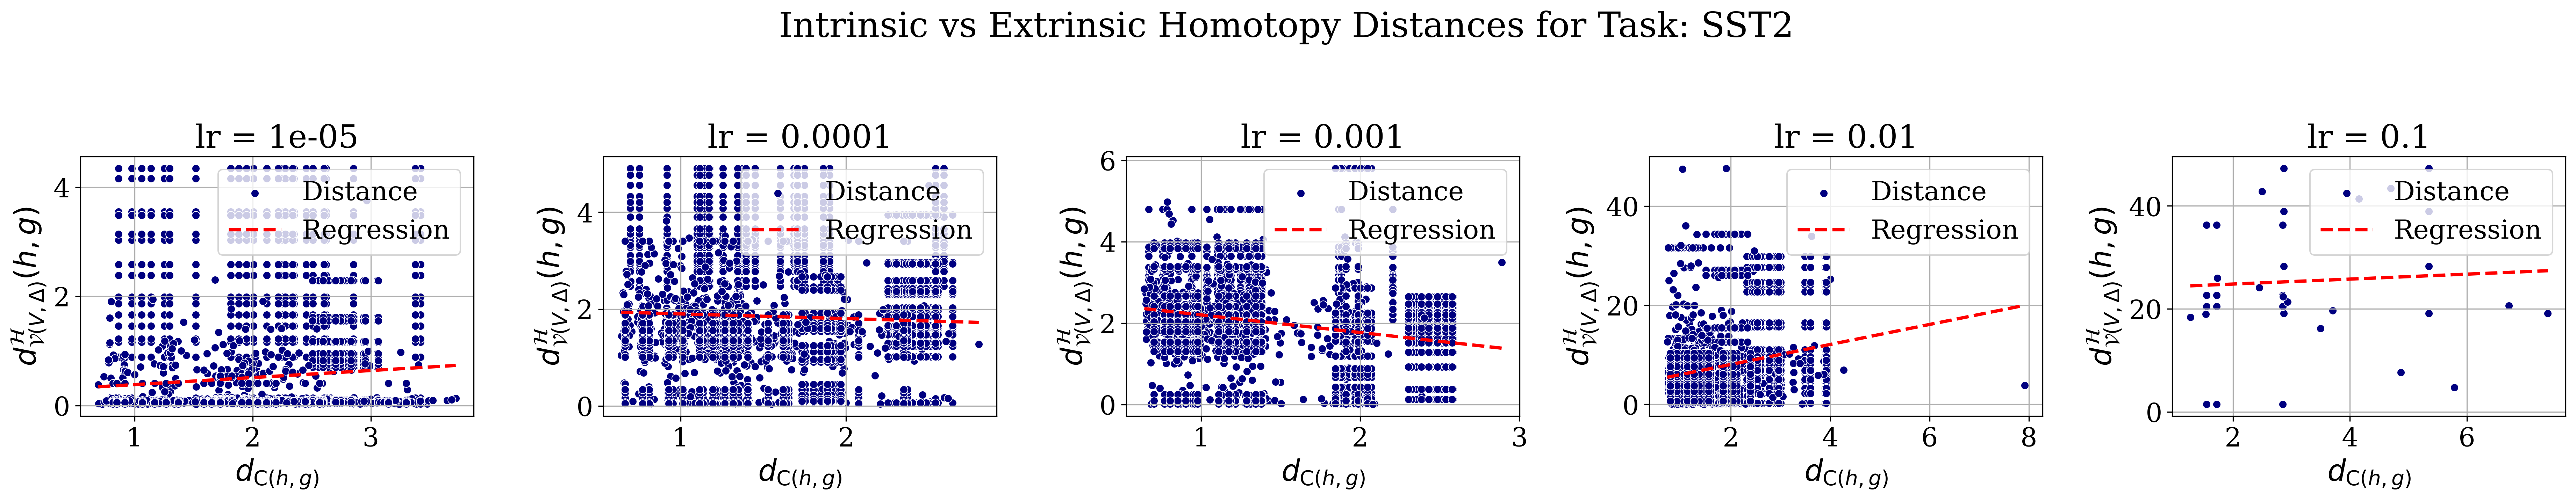
\includegraphics[width=\linewidth]{Abschlussarbeit/Pictures/intrinsic_vs_extrinsic_point_plots/PräsiDist_extr_intr_subplots_sst2.png}
	\caption{Intrinsic vs. extrinsic distances for encoder pairs on \texttt{SST-2}.}
	\label{fig:intrinsic_vs_extrinsic_sst2}
\end{figure}


For \texttt{SST-2}, we observe very low extrinsic distances for all encoder pairs at low learning rates, with no clear dependence on intrinsic distance.  
The regression lines are flat or slightly negative across learning rates \( \leq 10^{-3} \), suggesting that structurally dissimilar encoders can be aligned well in terms of task output.  
At higher learning rates (\( \geq 0.01 \)), extrinsic distances increase dramatically, while the correlation with intrinsic distance remains weak.  
This implies that for sentiment classification, intrinsic geometry does not reliably reflect task behavior, possibly due to sparse or high-level features driving classification.

\begin{figure}[H]
	\centering
	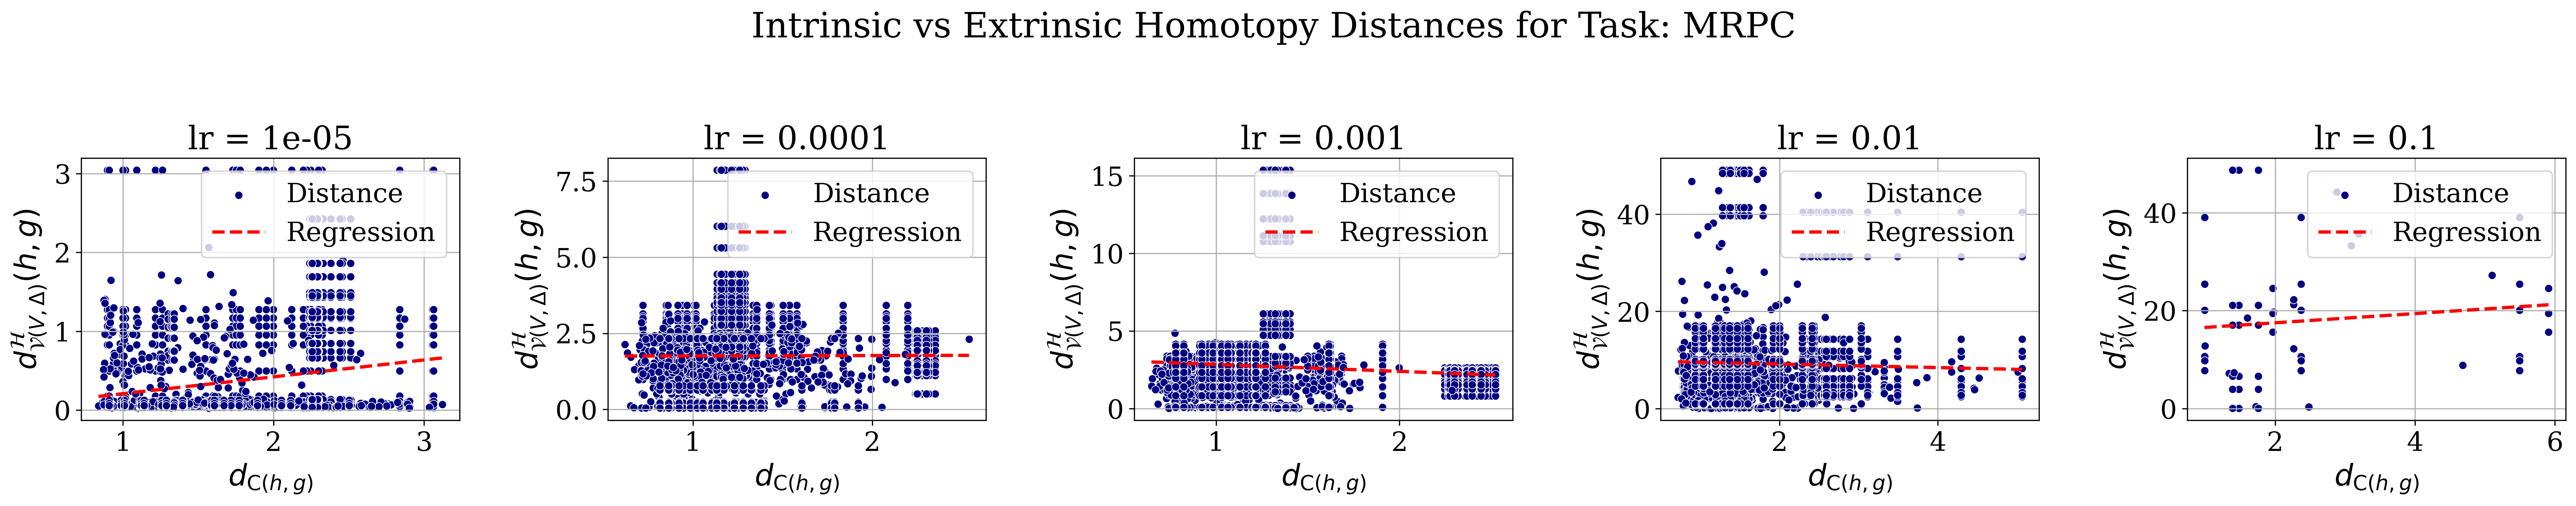
\includegraphics[width=\linewidth]{Abschlussarbeit/Pictures/intrinsic_vs_extrinsic_point_plots/PräsiDist_extr_intr_subplots_mrpc.png}
	\caption{Intrinsic vs. extrinsic distances for encoder pairs on \texttt{MRPC}.}
	\label{fig:intrinsic_vs_extrinsic_mrpc}
\end{figure}


The \texttt{MRPC} task lies between \texttt{SST-2} and \texttt{QNLI} in terms of alignment.  
At low learning rates, there is a moderate positive trend between intrinsic and extrinsic distance, with fewer extreme outliers than in \texttt{SST-2}.  
As learning rates increase, the variance in extrinsic distance grows, but the general trend persists, albeit more weakly.  
This suggests that representational similarity may be partially predictive of task behavior for paraphrase detection, but only under stable training conditions.

\begin{figure}[H]
	\centering
	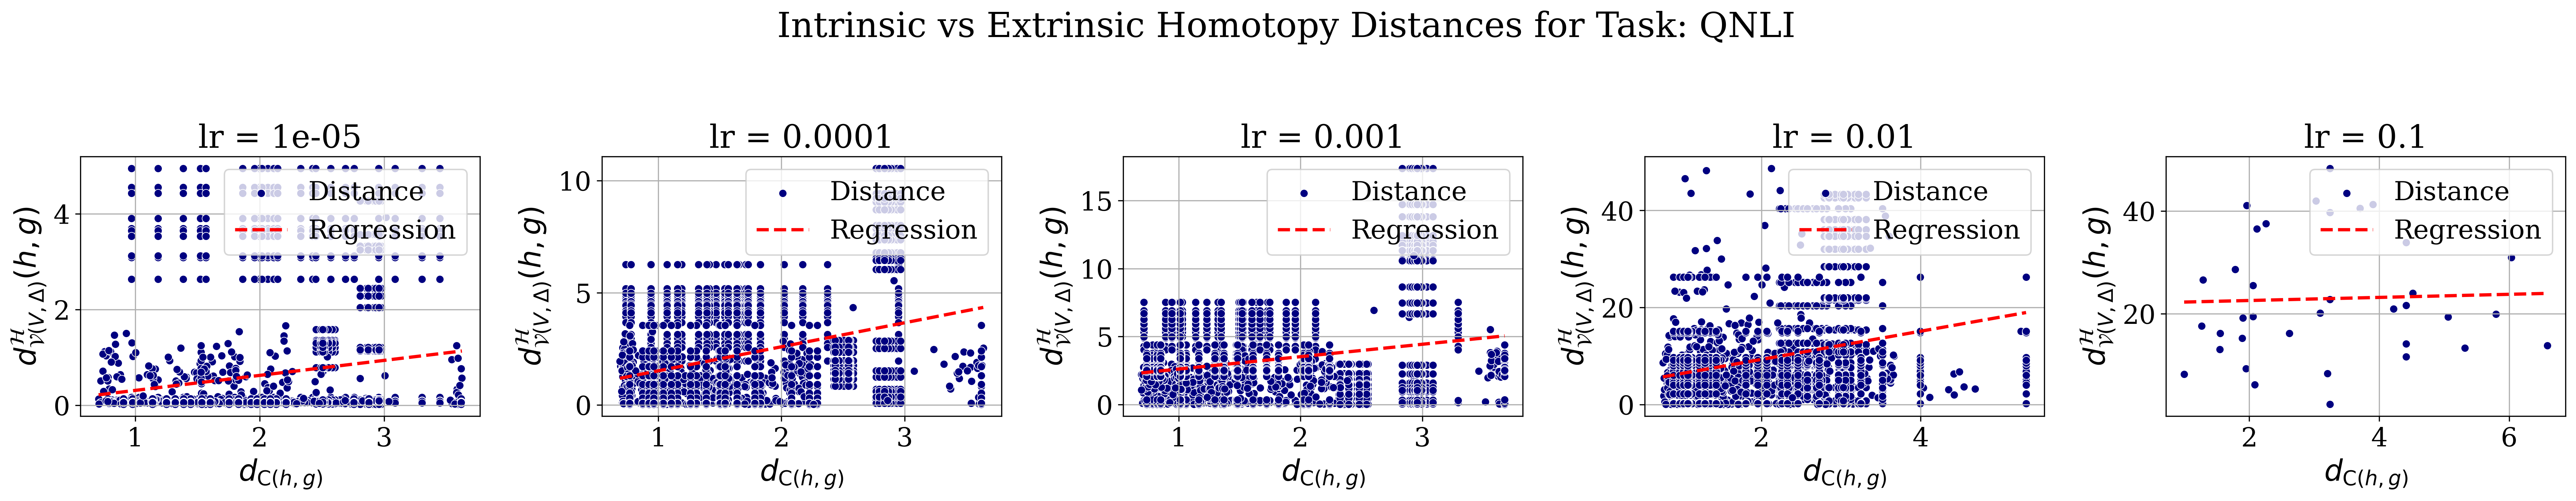
\includegraphics[width=\linewidth]{Abschlussarbeit/Pictures/intrinsic_vs_extrinsic_point_plots/PräsiDist_extr_intr_subplots_qnli.png}
	\caption{Intrinsic vs. extrinsic distances for encoder pairs on \texttt{QNLI}.}
	\label{fig:intrinsic_vs_extrinsic_qnli}
\end{figure}

\paragraph{QNLI.}
For \texttt{QNLI}, we observe a clear and consistent positive correlation between intrinsic and extrinsic distance across all learning rates.  
This indicates that encoders with similar internal representations also exhibit similar behavior on the task.  
Even at higher learning rates, where extrinsic distances increase, the regression slope remains positive and robust.  
This alignment may reflect the task's reliance on fine-grained semantic matching, which is more directly encoded in the latent space.


Overall, our findings demonstrate that the relationship between intrinsic and extrinsic homotopy is highly task-dependent.  
For some tasks, such as \texttt{QNLI}, intrinsic similarity can meaningfully predict downstream behavior.  
In others, like \texttt{SST-2}, functional similarity emerges independently of representational closeness.  
This suggests that structural alignment in representation space is neither necessary nor sufficient for downstream task alignment, and motivates task-aware evaluation of model similarity.

